\begin{pastexam}[label={px:ntu-108-comm-dsab-20}]{臺大電信所 108 學年度（B）第 20 題}
（單選；每題 2.5 分，答錯不倒扣）

Consider the AVL tree in Figure 1. After deleting key 12, what's the parent of the node with key 54?

A.~42 \qquad B.~66 \qquad C.~73 \qquad D.~87 \qquad E.~94

\begin{center}
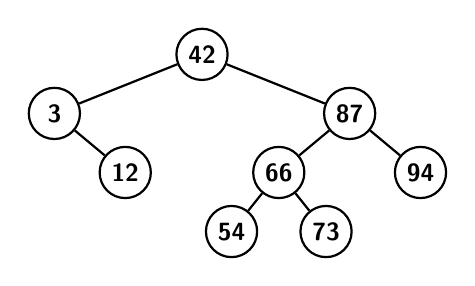
\begin{tikzpicture}[x=0.75cm,y=0.75cm,v/.style={circle,draw,thick,inner sep=0pt,minimum size=6.5mm,font=\sffamily\bfseries\small}]
\node[v] (n42) at (2.5,0) {42};
\node[v] (n3) at (0,-1) {3};
\node[v] (n87) at (5,-1) {87};
\node[v] (n12) at (1.2,-2) {12};
\node[v] (n66) at (3.8,-2) {66};
\node[v] (n94) at (6.2,-2) {94};
\node[v] (n54) at (3,-3) {54};
\node[v] (n73) at (4.6,-3) {73};
\draw[thick] (n42) -- (n3); \draw[thick] (n42) -- (n87); \draw[thick] (n3) -- (n12);
\draw[thick] (n87) -- (n66); \draw[thick] (n87) -- (n94);
\draw[thick] (n66) -- (n54); \draw[thick] (n66) -- (n73);
\end{tikzpicture}\\
Figure 1: AVL Tree
\end{center}
\end{pastexam}

\begin{pastsoln}
答案是 A。

從 Figure 1 的原樹刪除（和上一題的插入無關）。 $12$ 是葉節點，直接拿掉，$3$ 變成高度 $0$ 的葉節點。
往上檢查：$42$ 的左子樹高度 $0$、右子樹（$87$）高度 $2$，平衡因子 $-2$，\textbf{失衡}。

決定旋轉的種類看較高那一邊的子節點 $87$：它的左子樹 $66$ 高度 $1$、右子樹 $94$ 高度 $0$，
平衡因子 $+1$，是 RL 型（資結書第~10.2.6~節），要做雙旋轉：先在 $87$ 右旋、再在 $42$ 左旋，結果
是 $66$ 升到根，$42$ 和 $87$ 分別當它的左、右子節點；$66$ 原本的左子樹 $54$ 改掛成 $42$ 的右子節點，
右子樹 $73$ 改掛成 $87$ 的左子節點。
\begin{center}
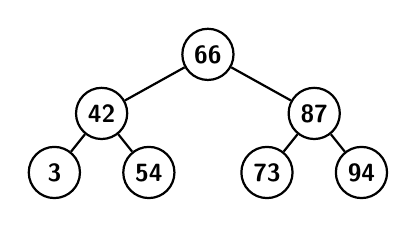
\begin{tikzpicture}[x=0.75cm,y=0.75cm,v/.style={circle,draw,thick,inner sep=0pt,minimum size=6.5mm,font=\sffamily\bfseries\small}]
\node[v] (n66) at (3,0) {66};
\node[v] (n42) at (1.2,-1) {42};
\node[v] (n87) at (4.8,-1) {87};
\node[v] (n3) at (0.4,-2) {3};
\node[v] (n54) at (2,-2) {54};
\node[v] (n73) at (4,-2) {73};
\node[v] (n94) at (5.6,-2) {94};
\draw[thick] (n66) -- (n42); \draw[thick] (n66) -- (n87);
\draw[thick] (n42) -- (n3); \draw[thick] (n42) -- (n54);
\draw[thick] (n87) -- (n73); \draw[thick] (n87) -- (n94);
\end{tikzpicture}
\end{center}
每個節點都平衡了，樹高從 $3$ 變成 $2$。 $66$ 是新的根，沒有更上面的祖先要檢查。 $54$ 的父節點是
$42$，選 A。 B 的 $66$ 是刪除前的父節點；只做一次左旋（把 $87$ 拉上來）的話，$66$ 整棵子樹會改掛到
$42$ 的右邊，$42$ 的高度變成 $2$，新的根 $87$ 左高 $2$、右高 $0$，仍然失衡，所以 RL 型一定要雙旋轉。
\end{pastsoln}
